\documentclass{article}

% set font encoding for PDFLaTeX, XeLaTeX, or LuaTeX
\usepackage{ifxetex,ifluatex}

\if\ifxetex T\else\ifluatex T\else F\fi\fi T%
  \usepackage{fontspec}
\else
  \usepackage[T1]{fontenc}
  \usepackage[utf8]{inputenc}
  \usepackage{lmodern}
\fi

\usepackage{amsmath}
\usepackage{amssymb}
\usepackage{amsthm}
\usepackage{bm}
\usepackage{mathtools}
\usepackage{physics}

\usepackage{enumitem}
\usepackage{multicol}
\usepackage{graphicx}
\usepackage{hyperref}
\usepackage[parfill]{parskip}
\usepackage{lipsum}
\usepackage[export]{adjustbox}

\usepackage{xparse} 
\usepackage{subfig} 
\usepackage{xparse} 
\usepackage{float}

\usepackage{biblatex} 

%%%%%This is an image table command, can likely be deleted
\newcommand{\subf}[2]{

%
{\small 
\begin{tabular}
  [t]{@{}c@{}} #1\ 
  \#2 
\end{tabular}
}

%
} 

\makeatletter
\renewcommand*\env@matrix[1][c]{\hskip -\arraycolsep
  \let\@ifnextchar\new@ifnextchar
  \array{*\c@MaxMatrixCols #1}}
\makeatother
%%%%%% Tensor Product
\NewDocumentCommand{\tens}{e{_^}}{ 
\mathbin{\mathop{\otimes}\displaylimits \IfValueT{#1}{_{#1}} \IfValueT{#2}{^{#2}} }}
%%%%%% Add \R Reals
\newcommand{\R}{\mathbb{R}} 
%%%%%% Add \theorem float
\newtheorem{theorem}{Theorem}
%%%%%% Add \definition float
\theoremstyle{definition} 
\newtheorem{definition}{Definition}[section]
%%%%%%%%%%%%%%%%%%%%%%%%%%%%%%%%%%%%%%%%%%%%%%%%%%%%%%%%%%%%%%%%%%%%%%%%%%%%%%%%%%%%%%%%%%%%%%%%%%%%%%%%%%%%%%%%%%%%%%%%%%
%%%%%Uncomment to add citation library 
\bibliography{lib} 
\title{Summary Report}
\author{Francesca Basini, David Helekal,\\Melissa Iacovidou, Swetha Usha Lal, Yiping Zhang}

\begin{document}
\maketitle
\newpage
\section{Model}

Let us define a $k$-age group compartmental SIRV model for the infection dynamics of the diseases covered by the MMR vaccine. This model takes the form of a system of four vectorised ordinary differential equations. Each of the $k$ vector entries then corresponds to a given age subgroup with span $a_i, \quad i\in1...k$. Each equation then governs the dynamics what proportion of the subpopulations is susceptible, infected, recovered, or of those who have been vaccinated.\\
The model can either be represented in matrix form
\begin{align*}
&\frac{d\mathbf{s}}{dt} &=&& \mathbf{B} - (\mathbf{V} + \mathbf{d})\mathbf{s} - \mathbf{s}*(\pmb{\beta}(t)\mathbf{C}\mathbf
{i})+\delta_{t_{end}}(t)\mathbf{A}\mathbf{s}\\
%%%%%%%%%%%%%%%%%%%%%%%%%%%%%%%%%%%%%%%%%%%%%%%%%%%%%%%%%%%%%%%%%%%%%%%%%%%%%%%%%%%%%%%%%%%%%%%%%%%%%%%%%%%%%%%%%%%%%%%%%%
&\frac{d\mathbf{i}}{dt} &=&&\mathbf{s}*(\pmb{\beta}(t)\mathbf{C}\mathbf{i}) - (\mathbf{d} + \pmb{\gamma})\mathbf{i}+\delta_{t_{end}}(t)\mathbf{A}\mathbf{i}\\
%%%%%%%%%%%%%%%%%%%%%%%%%%%%%%%%%%%%%%%%%%%%%%%%%%%%%%%%%%%%%%%%%%%%%%%%%%%%%%%%%%%%%%%%%%%%%%%%%%%%%%%%%%%%%%%%%%%%%%%%%%
&\frac{d\mathbf{r}}{dt} &=&& \pmb{\gamma}\mathbf{i} - \mathbf{d}\mathbf{r}+\delta_{t_{end}}(t)\mathbf{A}\mathbf{r}\\
%%%%%%%%%%%%%%%%%%%%%%%%%%%%%%%%%%%%%%%%%%%%%%%%%%%%%%%%%%%%%%%%%%%%%%%%%%%%%%%%%%%%%%%%%%%%%%%%%%%%%%%%%%%%%%%%%%%%%%%%%%
&\frac{d\mathbf{v}}{dt} &=&& \mathbf{V}\mathbf{s}-\mathbf{d}\mathbf{v} +\delta_{t_{end}}(t)\mathbf{A}\mathbf{v}\\
%%%%%%%%%%%%%%%%%%%%%%%%%%%%%%%%%%%%%%%%%%%%%%%%%%%%%%%%%%%%%%%%%%%%%%%%%%%%%%%%%%%%%%%%%%%%%%%%%%%%%%%%%%%%%%%%%%%%%%%%%%
\end{align*}
$\mathbf{s}*\mathbf{i}\quad\textit{Denotes the elementwise product}$\\
Where:
\begin{align*}
&\mathbf{s}, \mathbf{i}, \mathbf{r} ,\mathbf{v}\in \mathbb{R}^k& \quad& \text{k-age group compartment vectors}\\
%%%%%%%%%%%%%%%%%%%%%%%%%%%%%%%%%%%%%%%%%%%%%%%%%%%%%%%%%%%%%
%%%%%%%%%%%%%%%%%%%%%%%%%%%%%%%%%%%%%%%%%%%%%%%%%%%%%%%%%%%%%
&\mathbf{B}:=diag(B,0,...,0)& \quad& \text{Birth rate}\\
%%%%%%%%%%%%%%%%%%%%%%%%%%%%%%%%%%%%%%%%%%%%%%%%%%%%%%%%%%%%%
%%%%%%%%%%%%%%%%%%%%%%%%%%%%%%%%%%%%%%%%%%%%%%%%%%%%%%%%%%%%%
&\mathbf{V}:=diag(V_1,...,V_k) &\quad& \text{Vaccination rates}\\
%%%%%%%%%%%%%%%%%%%%%%%%%%%%%%%%%%%%%%%%%%%%%%%%%%%%%%%%%%%%%
%%%%%%%%%%%%%%%%%%%%%%%%%%%%%%%%%%%%%%%%%%%%%%%%%%%%%%%%%%%%%
&\mathbf{d}:=diag(d_1,...,d_k) &\quad& \text{Death rates due to other causes}\\
%%%%%%%%%%%%%%%%%%%%%%%%%%%%%%%%%%%%%%%%%%%%%%%%%%%%%%%%%%%%%
%%%%%%%%%%%%%%%%%%%%%%%%%%%%%%%%%%%%%%%%%%%%%%%%%%%%%%%%%%%%%
&\pmb{\beta}(t):=diag(\beta_1(t),...,\beta_k(t))&\quad& \text{Age-based force of infection}\\
%%%%%%%%%%%%%%%%%%%%%%%%%%%%%%%%%%%%%%%%%%%%%%%%%%%%%%%%%%%%%
%%%%%%%%%%%%%%%%%%%%%%%%%%%%%%%%%%%%%%%%%%%%%%%%%%%%%%%%%%%%%
&\pmb{\gamma}:=diag(\gamma_1,...,\gamma_k)&\quad&\text{Recovery rates}\\
%%%%%%%%%%%%%%%%%%%%%%%%%%%%%%%%%%%%%%%%%%%%%%%%%%%%%%%%%%%%%
%%%%%%%%%%%%%%%%%%%%%%%%%%%%%%%%%%%%%%%%%%%%%%%%%%%%%%%%%%%%%
&\mathbf{C}\in \mathbb{R}^{k\times k}, \mathbf{C} := (c)_{ij} &\quad& \text{\emph{Who Interacts With Who matrix}}\\
%%%%%%%%%%%%%%%%%%%%%%%%%%%%%%%%%%%%%%%%%%%%%%%%%%%%%%%%%%%%%
%%%%%%%%%%%%%%%%%%%%%%%%%%%%%%%%%%%%%%%%%%%%%%%%%%%%%%%%%%%%%
&\mathbf{A}\in\mathbb{R}^{k\times k}&\quad& \text{The age group transition matrix}
\end{align*}

  where $\mathbf{A}$ has the structure
\begin{gather*}
\mathbf{A}=\begin{bmatrix}[r]
 -a_1^{-1} &            &           &              &   \\
  a_1^{-1} &  -a_2^{-1} &           &              &   \\
           &  a_2^{-1}  & -a_3^{-1} &              &   \\
           &            & \ddots    & \ddots       &   \\
           &            &		        & a_{k-1}^{-1} & 0 \\
\end{bmatrix}
\end{gather*}
%%%%%%%%%%%%%%%%%%%%%%%%%%%%%%%%%%%%%%%%%%%%%%%%%%%%%%%%%%%%%
%%%%%%%%%%%%%%%%%%%%%%%%%%%%%%%%%%%%%%%%%%%%%%%%%%%%%%%%%%%%%
Or in indexed form
\begin{align*}
  &\frac{dS_{i}}{dt}&=&&\delta_1(i)B + \delta_{t_{end}}(t)a_{i-1}S_{i-1}-\sum_{j=1}^{k}\beta_{i}c_{ij}S_{i}I_{j}-(d_{i} + \delta_{t_{end}}(t)a_{i} + v_{i})S_{i}\\
  &\frac{dI_{i}}{dt} &=&&\delta_{t_{end}}(t)a_{i-1}I_{i-1}+\sum_{j=1}^{k}\beta_{i}c_{ij}S_{i}I_{j}-(d_{i}+\gamma_{i}+\delta_{t_{end}}(t)a_{i})I_{i}\\
  &\frac{dR_{i}}{dt} &=&& \delta_{t_{end}}(t)a_{i-1}R_{i-1}+\gamma_{i}I_{i}-(d_{i}-\delta_{t_{end}}(t)a_{i})R_{i}\\
  &\frac{dV_{i}}{dt} &=&& \delta_{t_{end}}a_{i-1}V_{i-1}+v_iS_i-d_{i}V_{i}-\delta_{t_{end}}(t)a_{i}V_{i}
\end{align*}
where $i=1...k$ and $a_0 = a_k = 0$.
\section{Data}
\subsection{Immunisation Rates}
Immunisation is available from the NHS COVER reports \cite{noauthor_childhood_nodate}.
\subsection{Between Group Contact Rates}
As a starting point for \emph{Who Interacts With Who} matrices, the POLYMOD study \cite{mossong_social_2008} can utilised. This matrix will then further be weighted by force of infection for each age group, to be inferred from data.
\subsection{Epidemiologic Data}
There are several sources of age-structured epidemiologic data for MMR diseases available.\\ By far the highest temporal resolution for measles and rubella is offered by the ECDC Surveillance Atlas of Infectious Diseases dataset \cite{noauthor_surveillance_nodate}, which offers age standardised rates with monthly resolution, spanning years 1999-2019 for measles, and 2007-2019 for rubella. Unfortunately for mumps this dataset only offers yearly resolution for years 2000-2017.\\
Further recent age-structured data with yearly temporal resolution is available from Public Health England (PHE) reports \cite{noauthor_confirmed_nodate,noauthor_mumps_nodate,noauthor_rubella_nodate}\\
Historic age-structured data can be obtained from the Health Protection Agency (HPA) archives \cite{noauthor_archived_nodate,noauthor_archived_nodate-1,noauthor_archived_nodate-2}. These datasets span years 1989-2012, and offer yearly temporal resolution. This data offers an insight into situation when vaccination rate too low to confer herd immunity.\\
This data should be sufficient to parametrise and fit an age-stratified SIRV model for years 1998-2019, as well as to confirm that the compound behaviour of this model under low vaccination rates corresponds to real data.
\begin{figure}
  \centering
  \subfloat[]{\label{dat:a}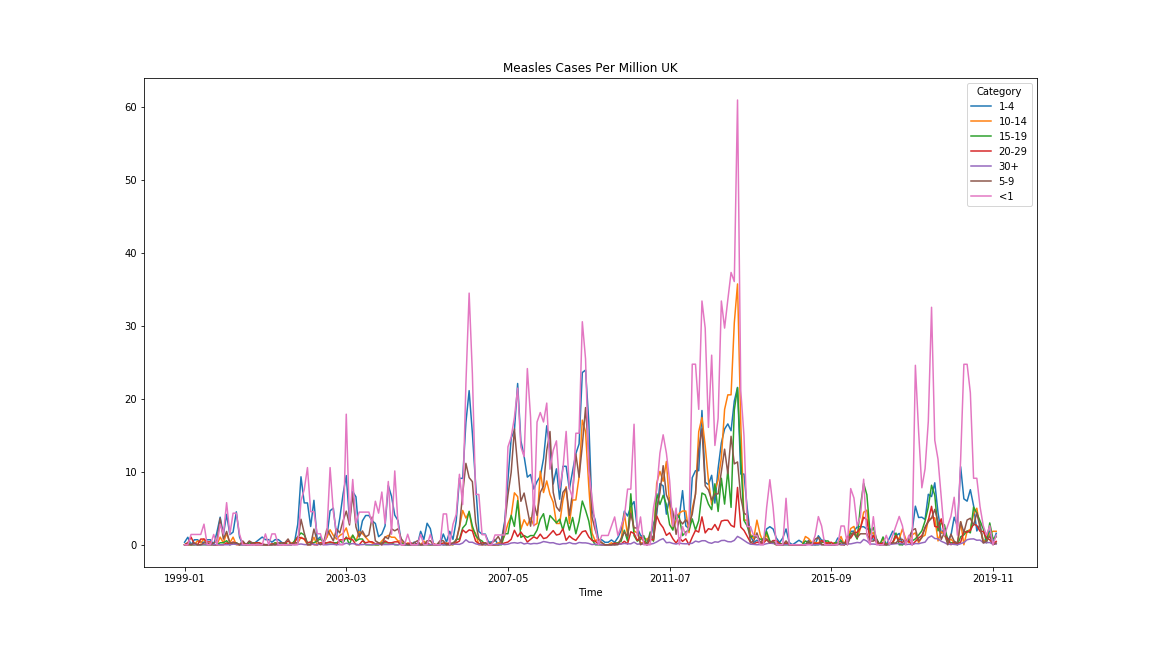
\includegraphics[scale=.22]{../data_nb/MeaslesPlot}}
  \par
  \centering
  \subfloat[]{\label{dat:b}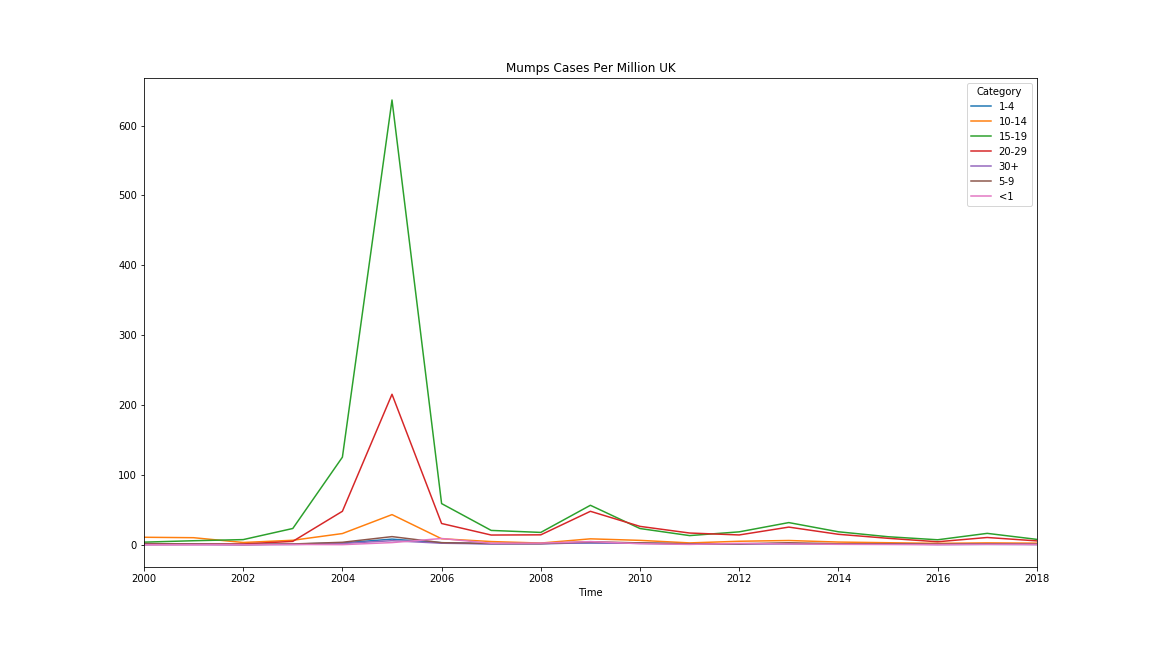
\includegraphics[scale=.22]{../data_nb/MumpsPlot}}
  \par
  \centering
  \subfloat[]{\label{dat:c}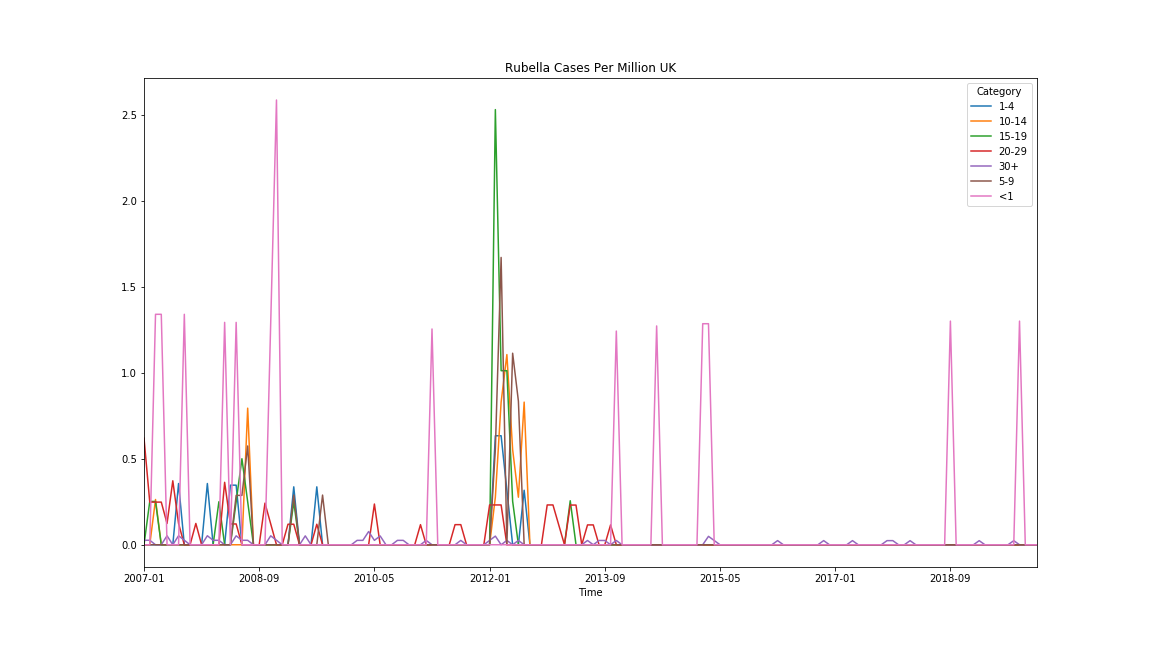
\includegraphics[scale=.22]{../data_nb/RubellaPlot}}
  \caption{ECDC Age Standardised rates for the UK plotted against time \ref{dat:a} Measles data \ref{dat:b} Mumps data \ref{dat:c} Rubella data}
  \label{fig:dat}
\end{figure}
\newpage
%%%%%should have a separate page for bibliography
\printbibliography  
\end{document}
